\subsection{乱数}

\subsubsection{一様乱数}
一様分布に従う乱数のこと。
一様分布のPDF、CDF、Quantileを図\ref{fig:uniform-pdf-cdf}に示す。
\begin{figure}
	\centering
	\begin{subfigure}{0.48\columnwidth}
		\centering
		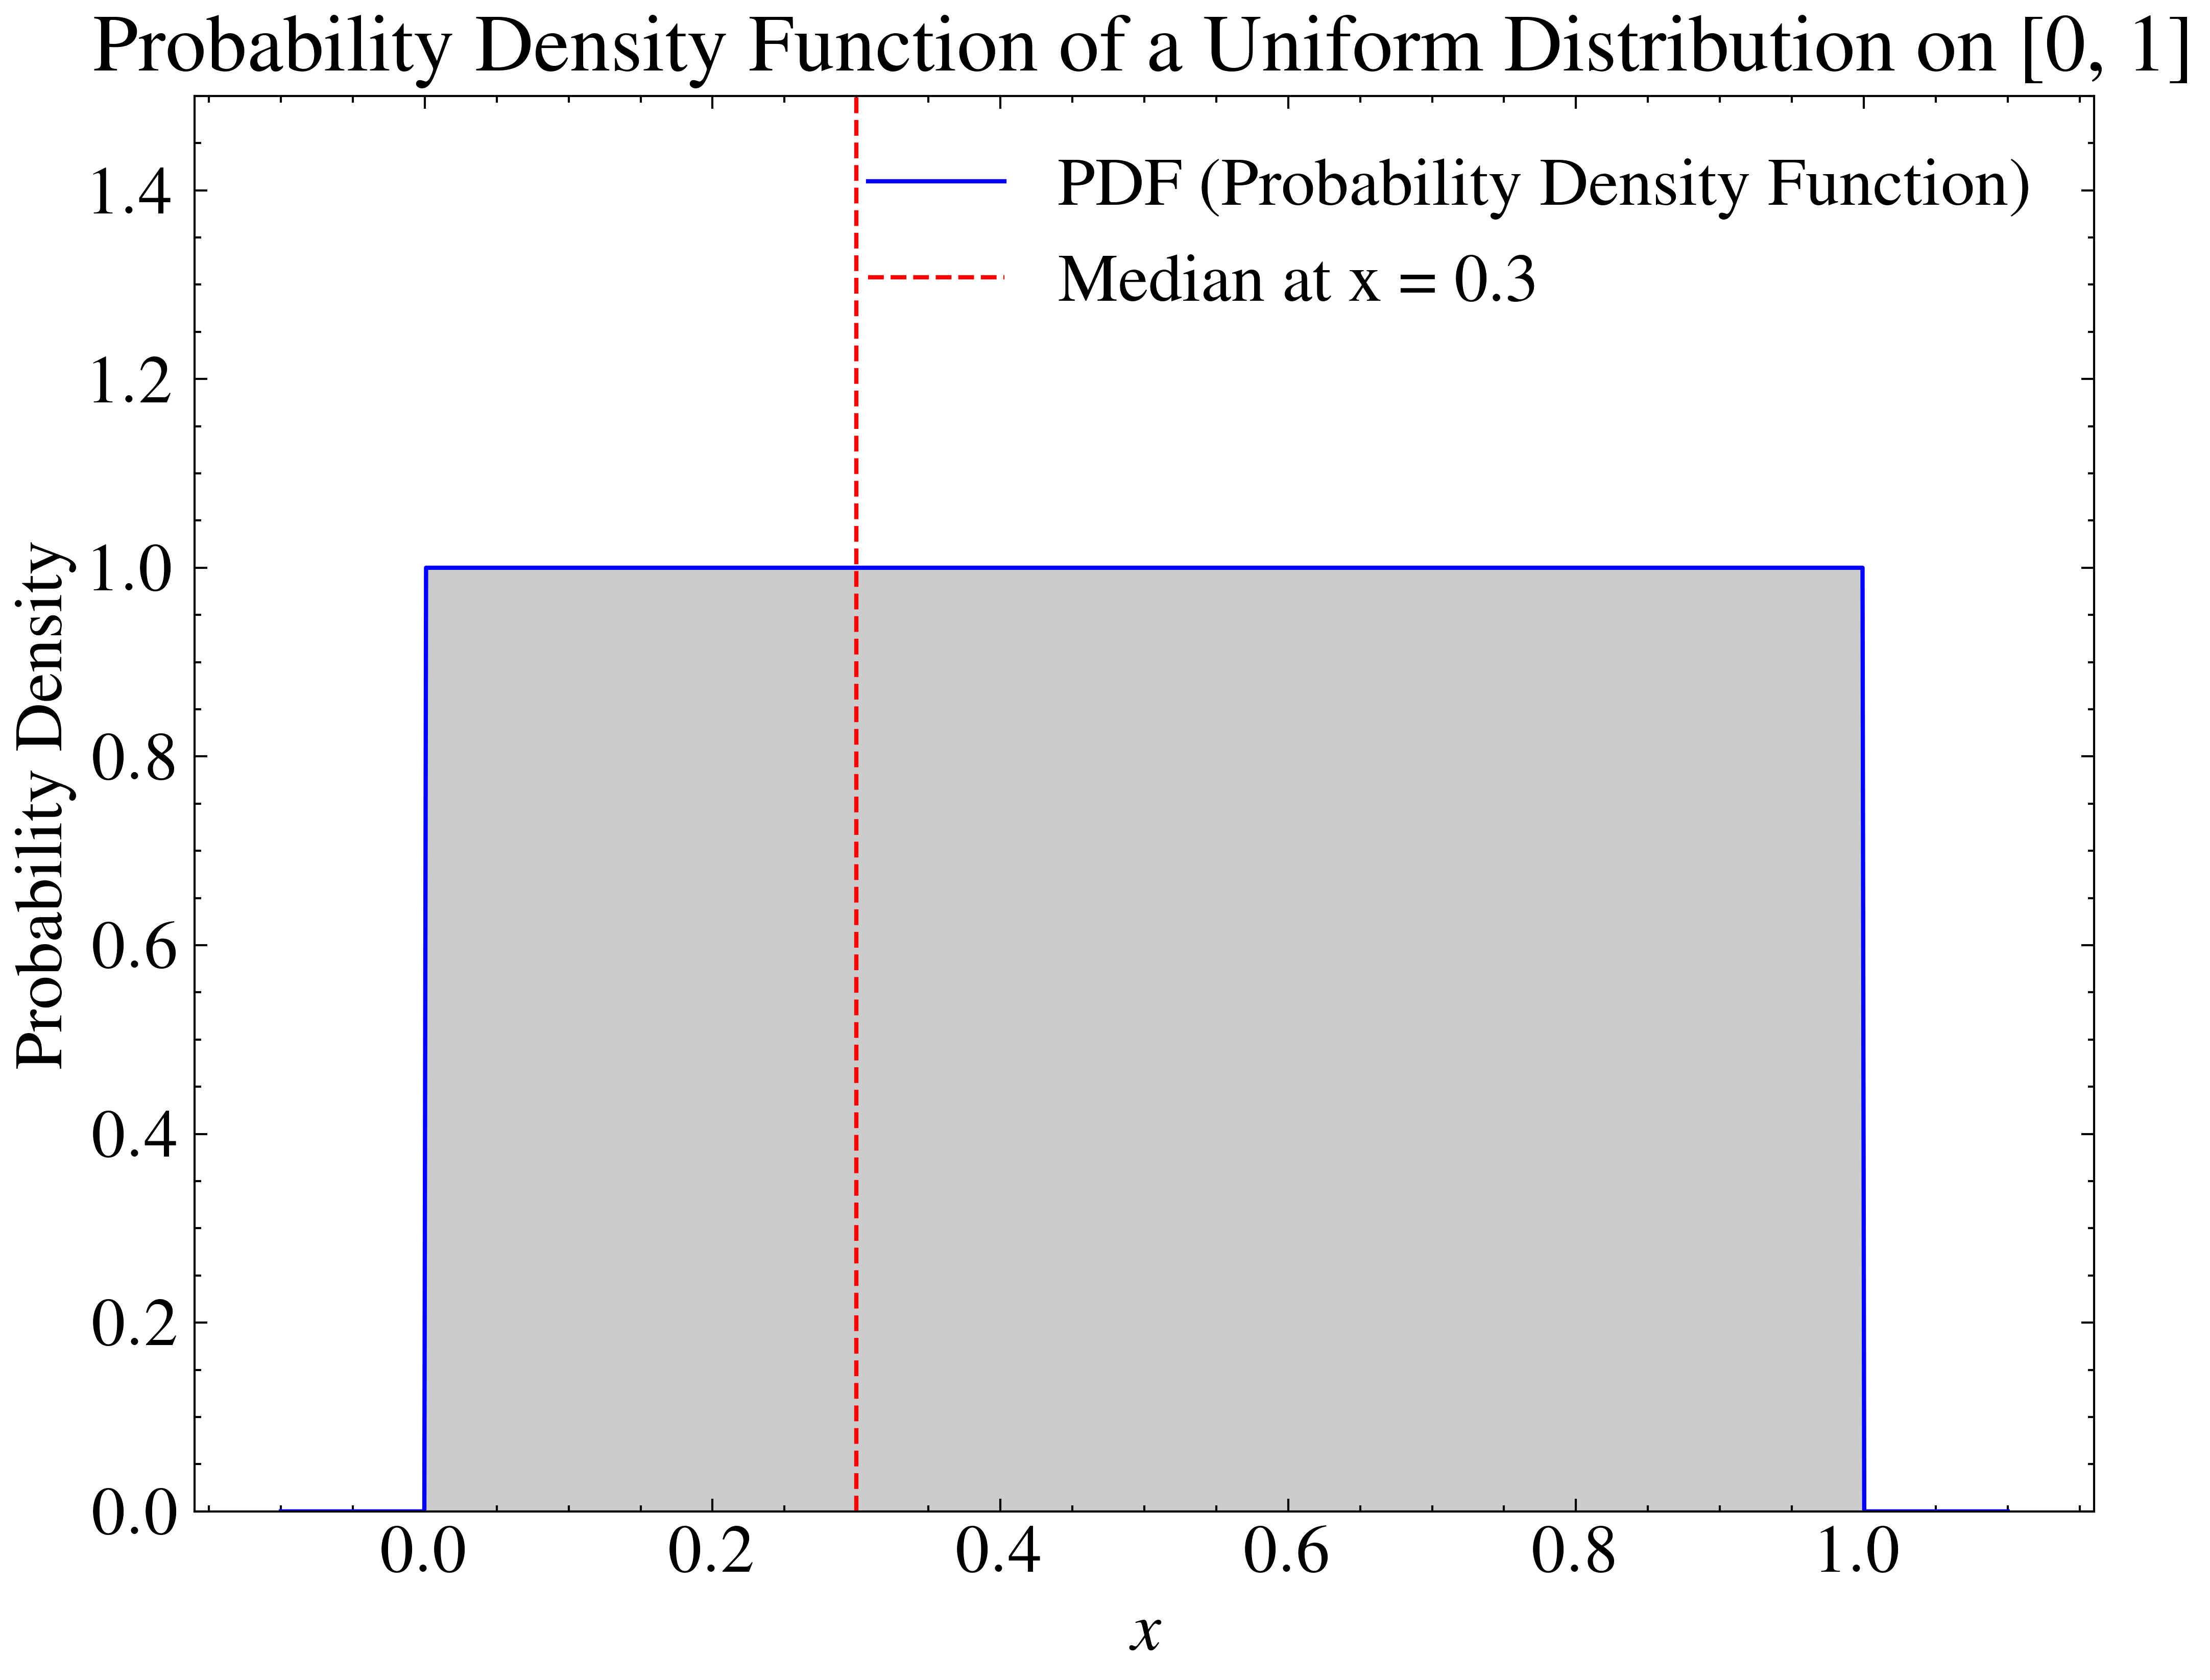
\includegraphics[width=0.8\linewidth]{src/figures/uniform-distribution-pdf-cdf-quantile/uniform_pdf.png}
		\subcaption{PDF}
	\end{subfigure}
	\begin{subfigure}{0.48\columnwidth}
		\centering
		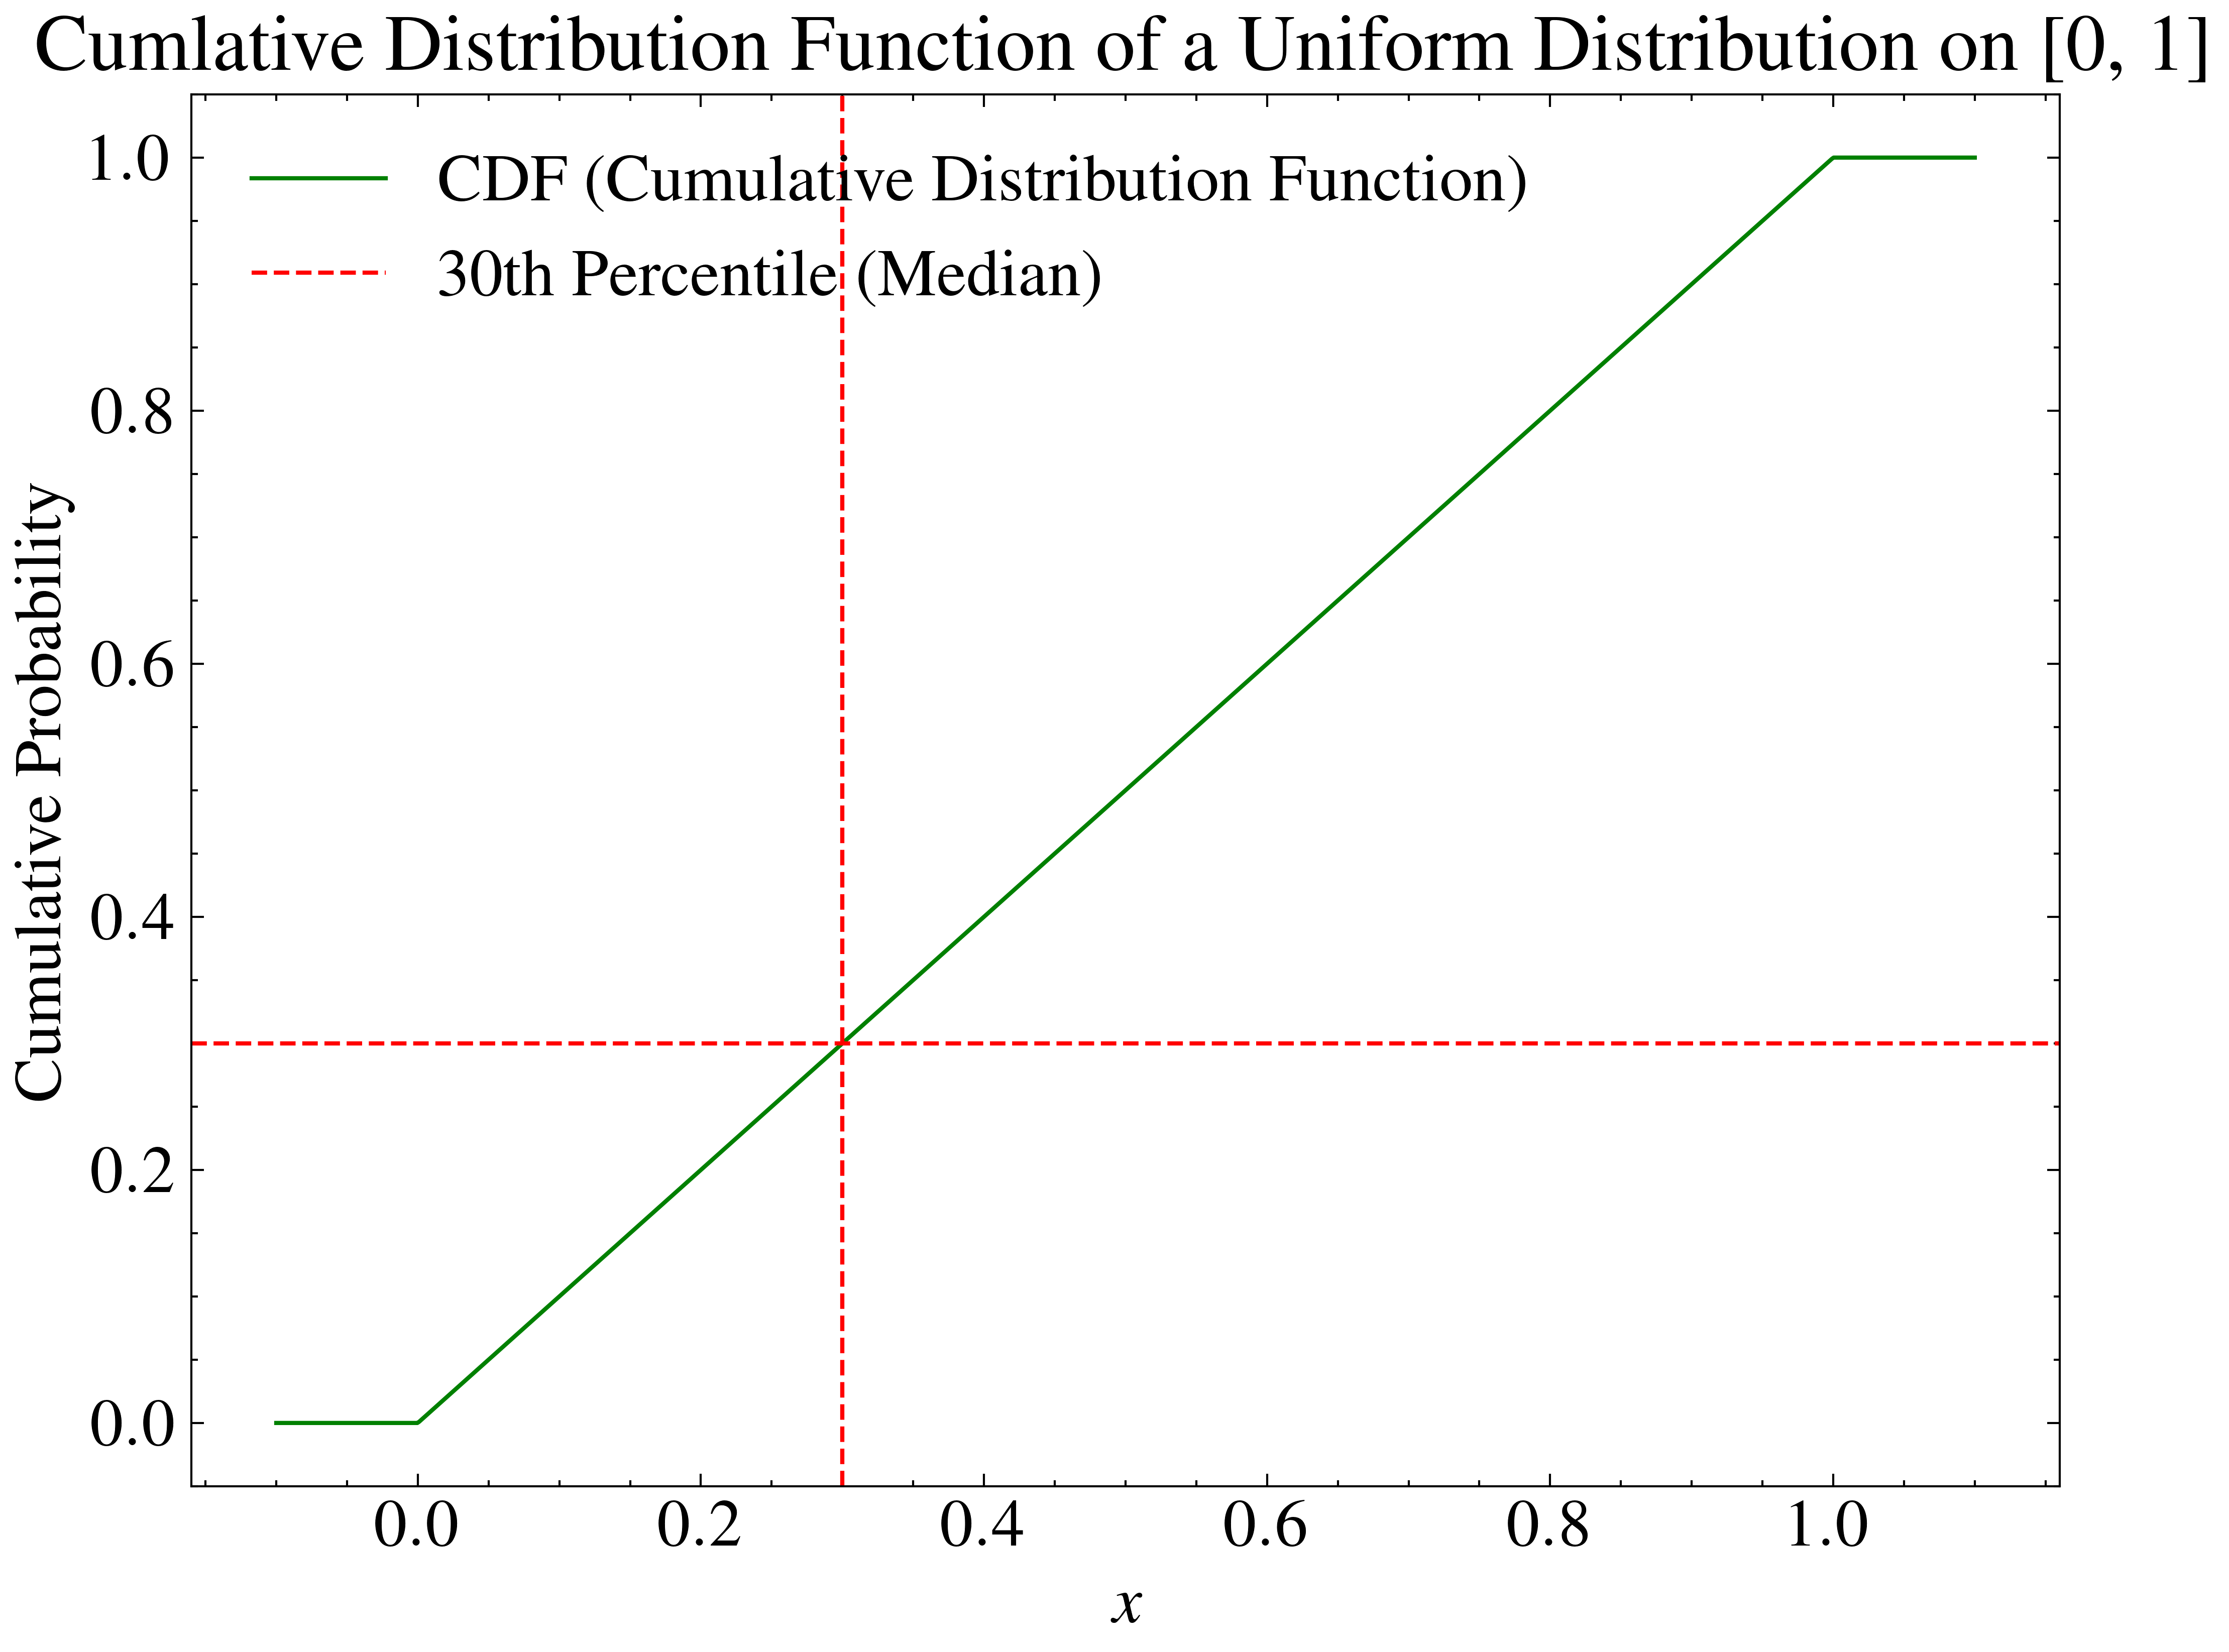
\includegraphics[width=0.8\linewidth]{src/figures/uniform-distribution-pdf-cdf-quantile/uniform_cdf.png}
		\subcaption{CDF}
	\end{subfigure}
	\caption{一様分布のPDFとCDF}\label{fig:uniform-pdf-cdf}
\end{figure}

一様乱数を生成するプログラムは数多く開発されてきたが、中でも最も早い時期に提案された方法が線形合同法である。
線形合同法は、次の漸化式
\begin{equation*}
	X_{n+1} = (aX_n + c) \mod m \,, n = 0, 1, 2, \ldots
\end{equation*}
を用いて、乱数列$X_0, X_1, X_2, \ldots$を生成する方法である。
この漸化式で表される乱数列は周期性をもち、それを長くするために$m$はできるだけ大きくとるのが普通である。
その結果、計算速度が遅くなり実用的でなくなった。

\subsubsection{正規乱数}
正規分布に従う乱数のこと。
正規分布は、平均$\mu$、分散$\sigma^2$の2つのパラメータで特徴づけられ、
\begin{equation*}
	\mathcal{N}(x) = \frac{1}{\sqrt{2\pi}\sigma} \exp\left(-\frac{(x-\mu)^2}{2\sigma^2}\right)
\end{equation*}
と表される。
特に、平均が0、分散が1の正規分布を標準正規分布と呼び、
\begin{equation}
	\mathcal{N}(x) = \frac{1}{\sqrt{2\pi}} \exp\left(-\frac{x^2}{2}\right)
\end{equation}
で表される。
この標準正規分布のPDF、CDF、Quantileは図\ref{fig:pdf-cdf-quantile}に示す。

\paragraph{逆関数法}
乱数変換のための一般的な方法である。
$F(x)$の逆関数
\begin{equation*}
	F^{-1}(y) = \inf\{x: F(x) \geq y \},\, 0 \leq y \leq 1
\end{equation*}
を用いて、
\begin{equation}\label{eq:inverse-function}
	X = F^{-1}(U)
\end{equation}
とすると、
\begin{equation*}
	\mathrm{Pr}\{X \leq x\} = \mathrm{Pr}\{F^{-1}(U) \leq x\} = \mathrm{Pr}\{U \leq F(x)\} = F(x)
\end{equation*}
となり、$X$は$F(x)$に従う乱数となる。


\paragraph{Box-Muller法}
Box-Muller法は、一様乱数を用いて正規乱数を生成する方法である。
具体的には、$[0, 1]$上の一様乱数$U_1, U_2$を用いて、
\begin{equation}\label{eq:box-muller}
	\begin{split}
		Z_1 & = \sqrt{-2\ln U_1} \cos(2\pi U_2) \\
		Z_2 & = \sqrt{-2\ln U_1} \sin(2\pi U_2)
	\end{split}
\end{equation}
とすると、$Z_1, Z_2$は独立な標準正規乱数となる。
以下に簡単な証明を示す。
まず、指数分布と一様分布で正規分布が得られることを示す。
$R$が$[0, 2]$の指数分布に従い、$\Theta$が$[0, 2\pi]$の一様分布に従うとし、
$Z_1 = \sqrt{R}\cos\Theta$、$Z_2 = \sqrt{R}\sin\Theta$とする。
$f$を$Z_1, Z_2$の同時確率密度関数、$g$を$R, \Theta$の同時確率密度関数とすると、
\begin{equation*}
	\begin{split}
		 & \text{$R$が$[0, 2]$の指数分布に従い、$\Theta$が$[0, 2\pi]$の一様分布に従う}                                \\
		 & \Leftrightarrow g(r, \theta) = \dfrac{1}{2\pi} \dfrac{1}{2} e^{-\frac{r}{2}}            \\
		 & \Leftrightarrow f(z_1, z_2) = \dfrac{1}{2\pi} \dfrac{1}{2} e^{-\frac{z_1^2 + z_2^2}{2}} \\
		 & \Leftrightarrow \text{$X_1$と$X_2$は独立な標準正規分布に従う}
	\end{split}
\end{equation*}
となる。
よって二つの独立な標準正規乱数$U_1, U_2$から、
\begin{equation*}
	\begin{split}
		R = -2\ln U_1 \\
		\Theta = 2\pi U_2
	\end{split}
\end{equation*}
とすれば、$Z_1, Z_2$は独立な標準正規乱数となる。
